\section{Experiments}
\begin{figure}
    \centering
    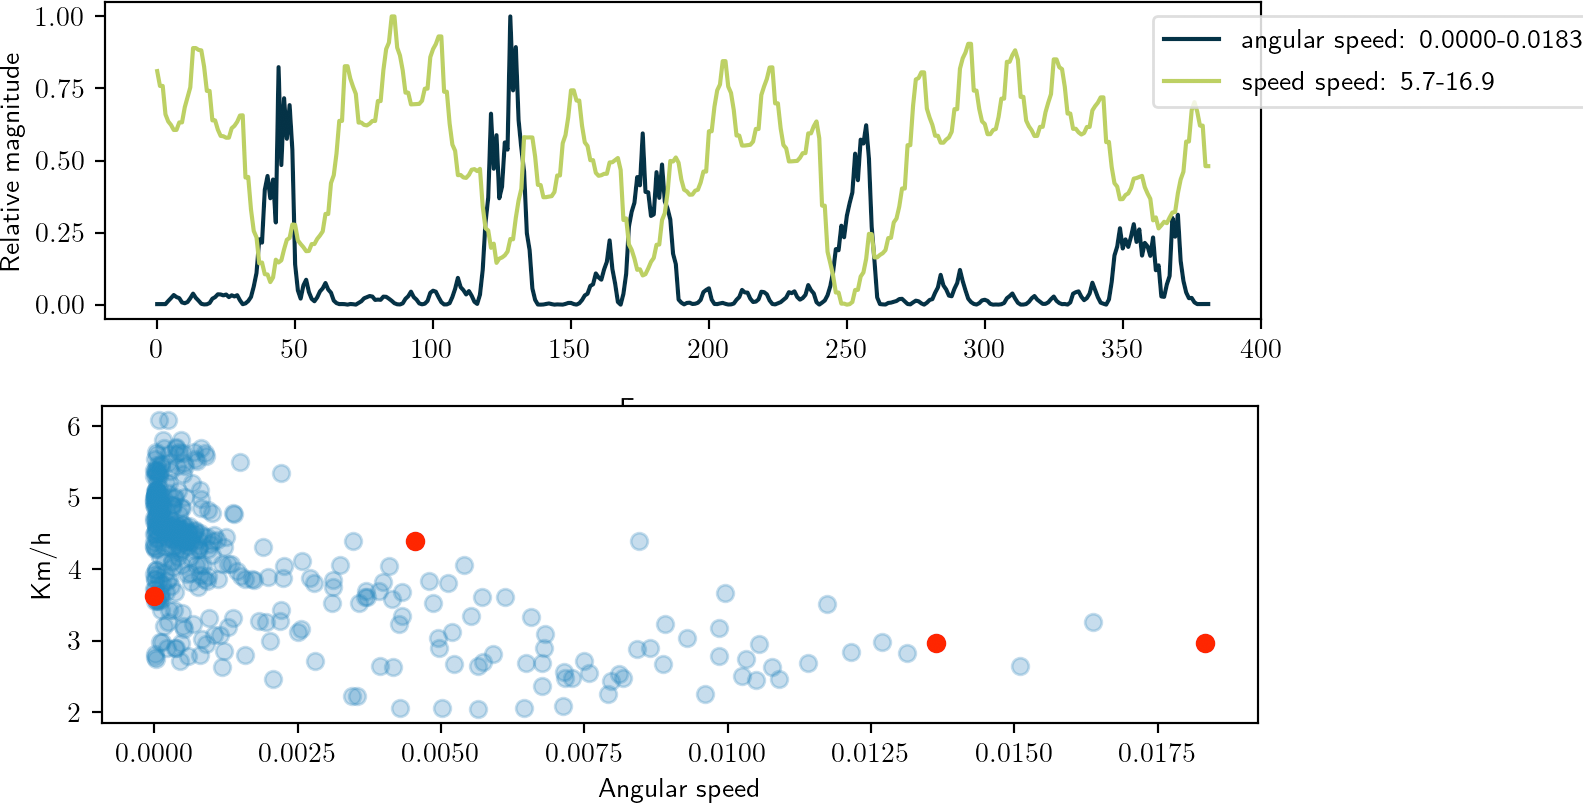
\includegraphics[width=1.0\columnwidth]{img/movement_stats.png}
    \caption{An animation with 5 90 degree turns has complex changes to speed and angular speed.}
    \label{fig:results:trajectory_estimation}
\end{figure}

A series of animations was recorded using the inertial sensor based XSens suit and a three human subjects. The raw sensor data was cleaned using the automatic post processing procedure available in the XSens MVN Animate Pro software application. Some artifacts remain.
The movement set was inspired by the structure of locomotion sets used in game production, and contains turns at various angles follow by straight movements. The subject was instructed to keep the movement consistent and to follow the various movements closely. More complex movements types such as vaulting, cover or response to perturbations have not been examined. Fig. \ref{fig:results:trajectory_estimation} illustrates the complexity of 90 degree turns. 

\subsection{Movement Characteristics}
\begin{figure}
    \centering
    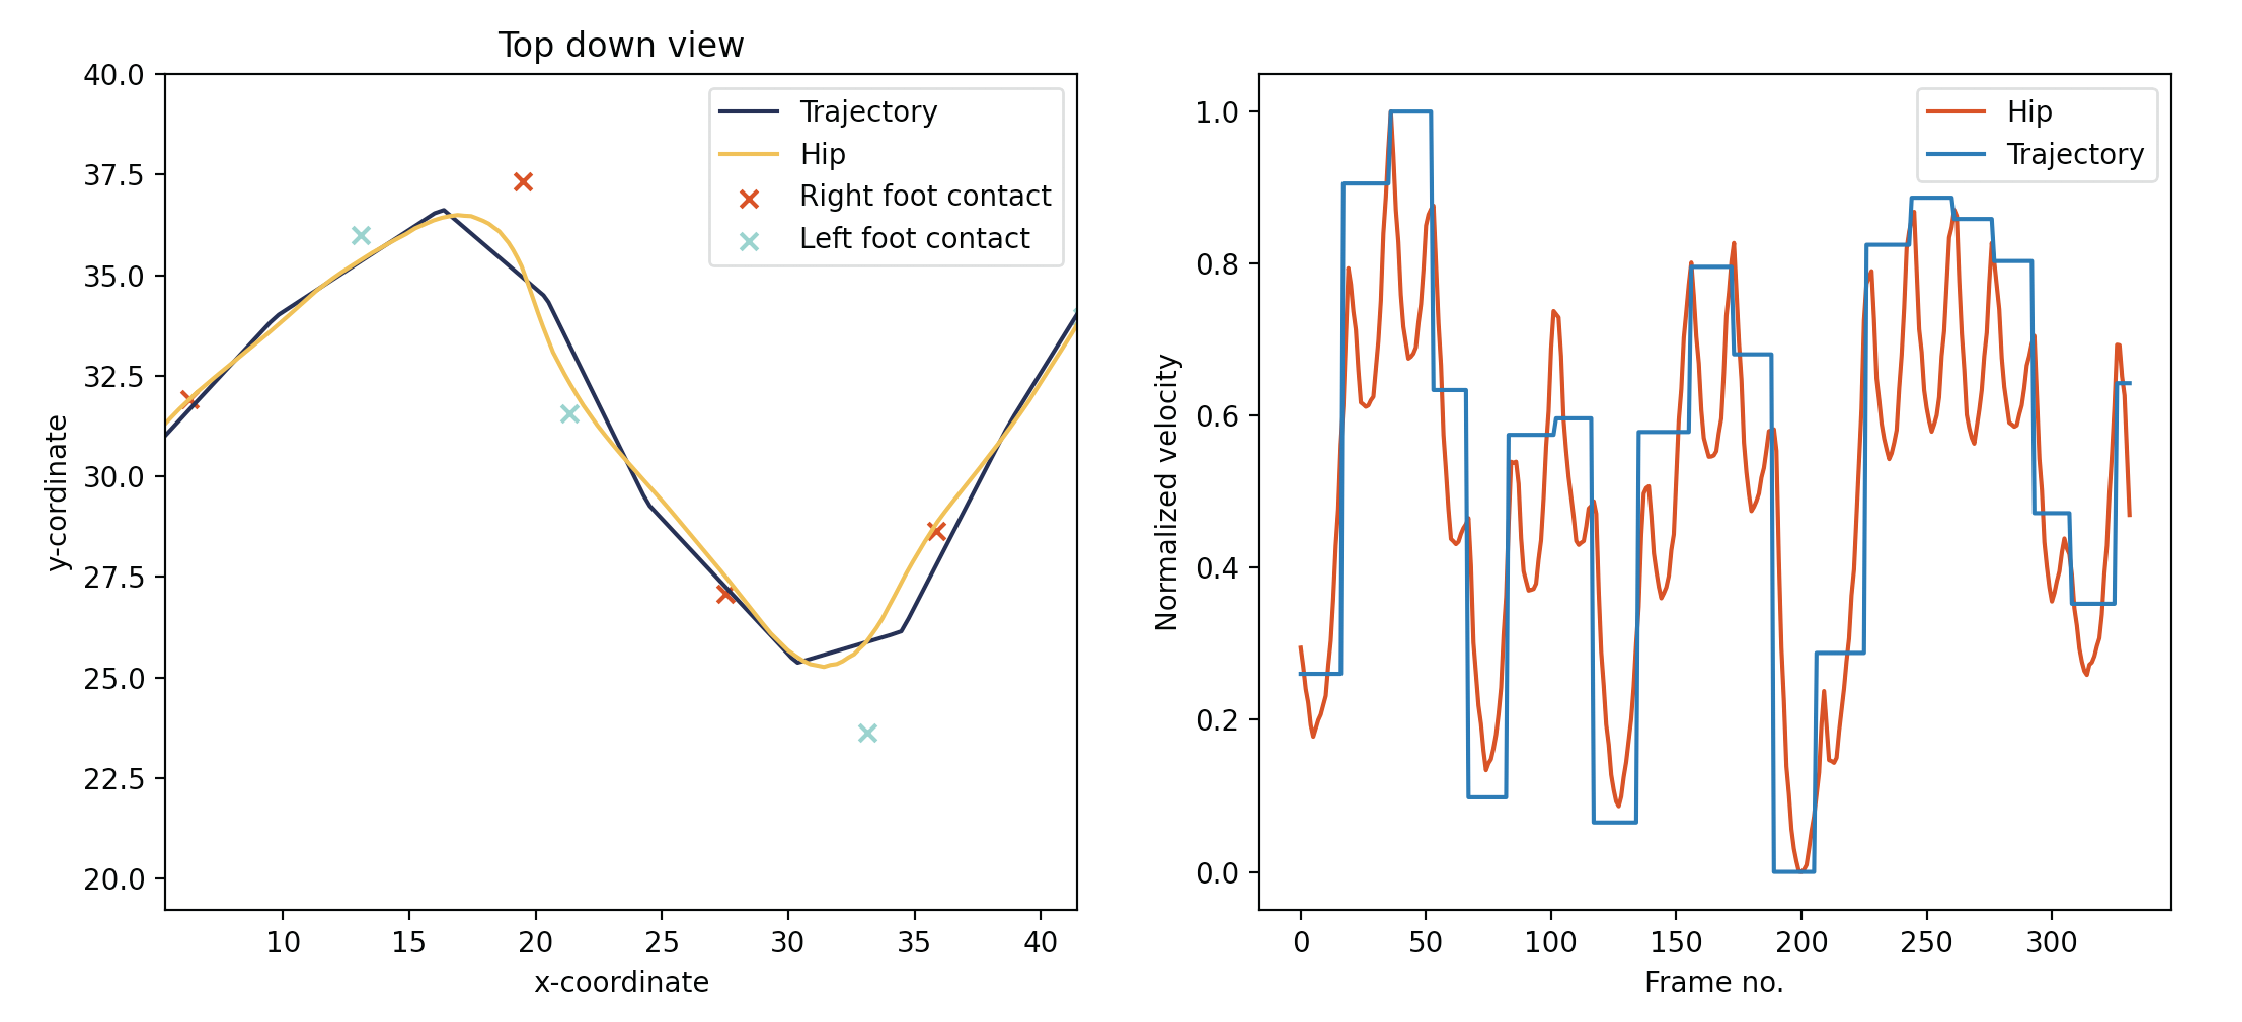
\includegraphics[width=1.0\columnwidth]{img/trajectory_estimation.png}
    \caption{Left plot shows hip movement cross back and forth between the estimated trajectory, and tangential directions sampled at individual positions hip give poor descriptions of the overall movement direction. Right plot show trajectories having more stable velocities.}
    \label{fig:results:trajectory_estimation}
\end{figure}

\begin{figure}
    \centering
    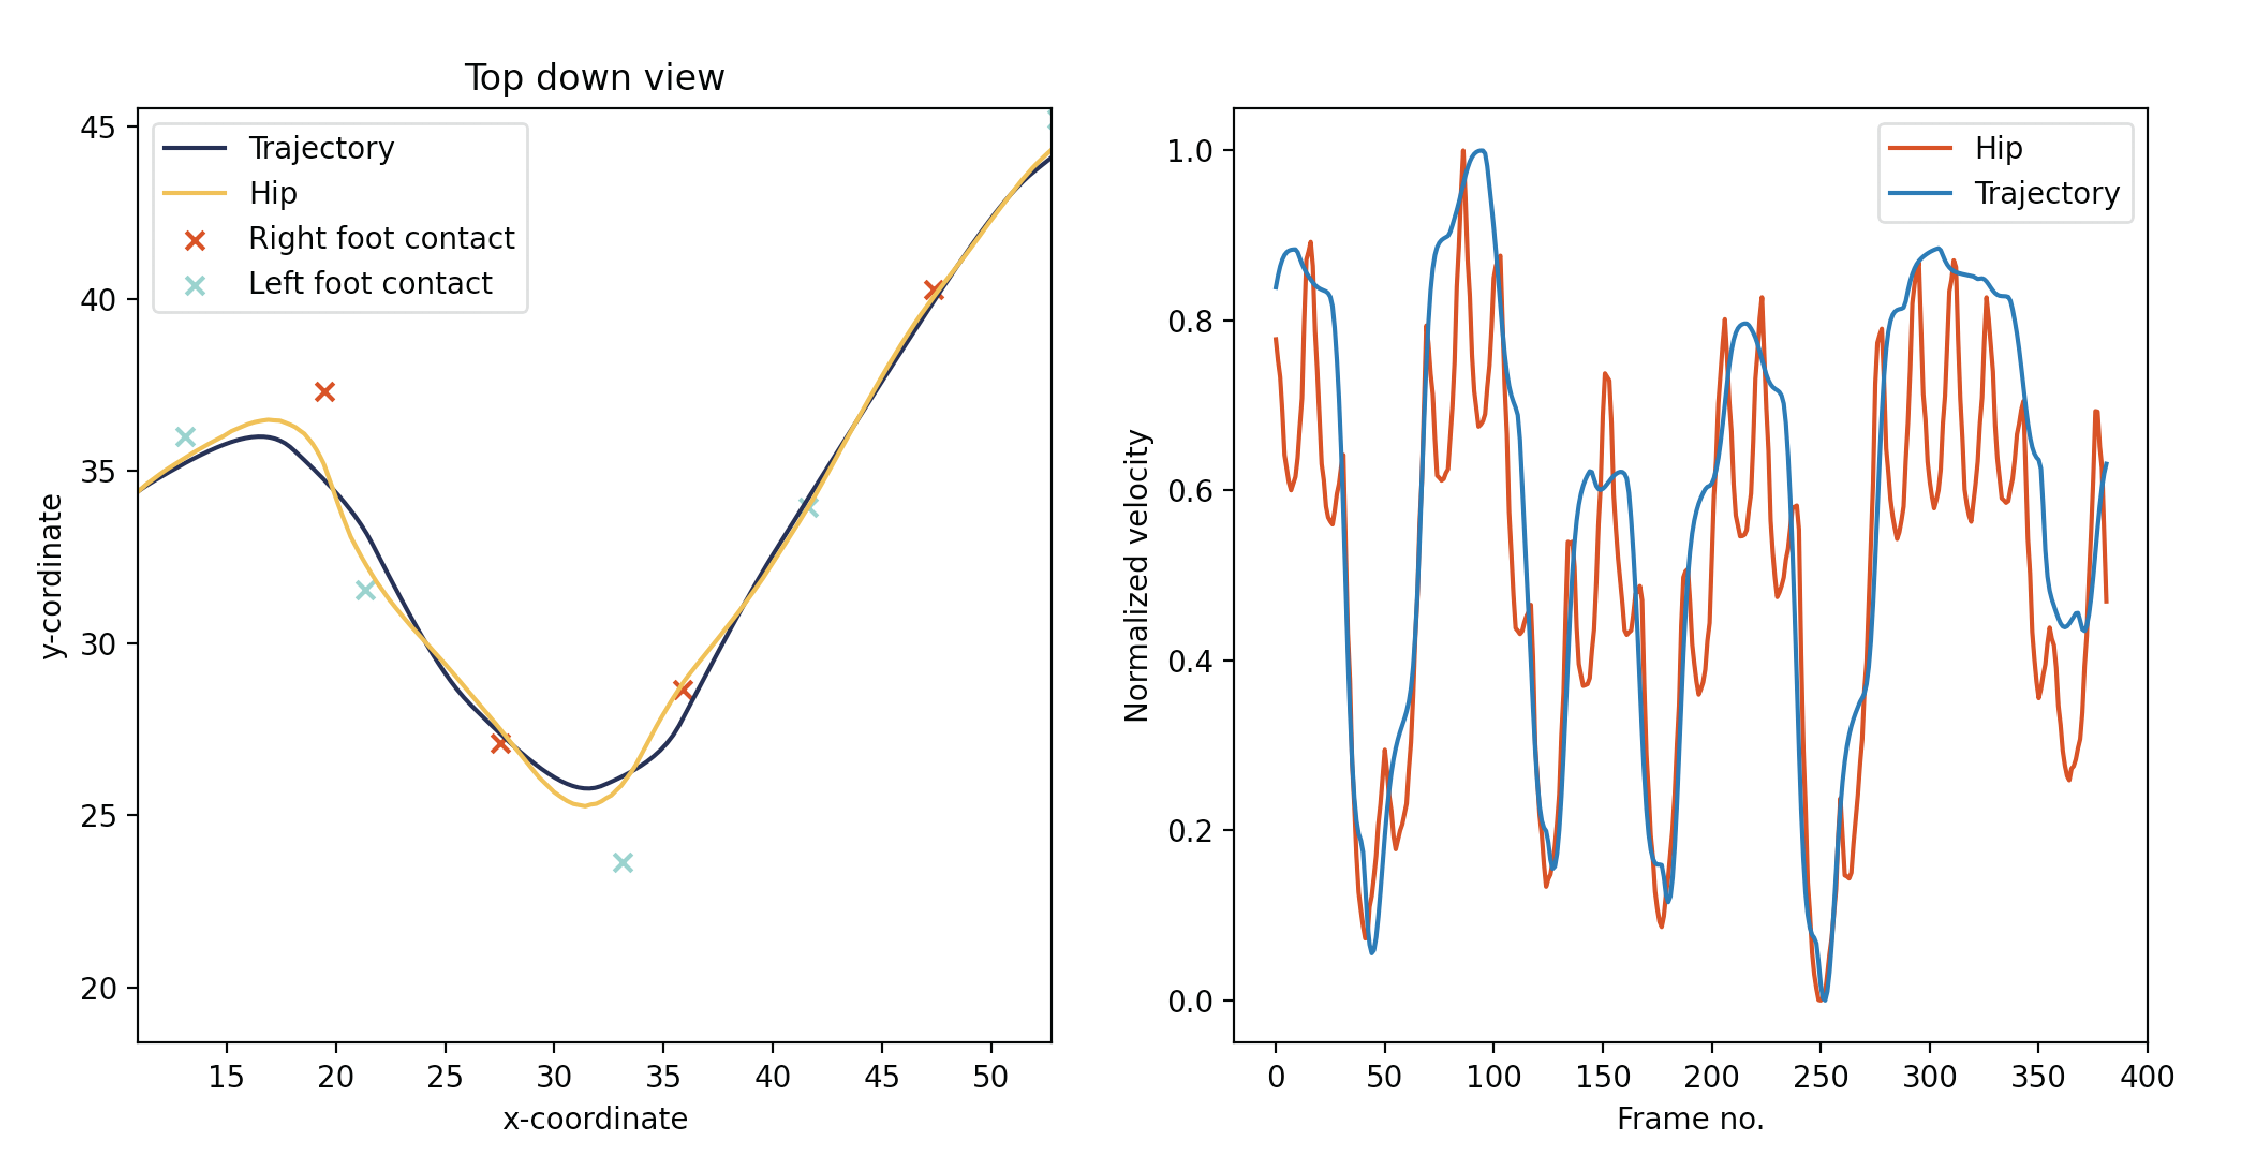
\includegraphics[width=1.0\columnwidth]{img/trajectory_estimation_smooth.png}
    \caption{By interpolation frame delta across foot contact dependent section, we achieve a smoother sampling of the trajectory. The smoothing is visible in both the path and the velocities.}
    \label{fig:results:trajectory_estimation_smooth}
\end{figure}

\begin{figure}
    \centering
    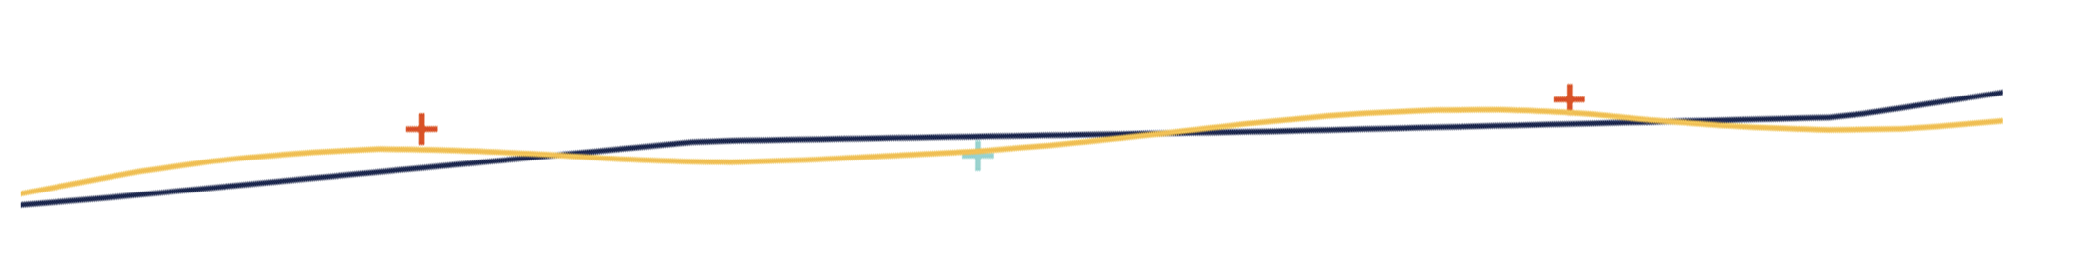
\includegraphics[width=1.0\columnwidth]{img/straight_trajectory.png}
    \caption{}
    \label{fig:results:trajectory_straight}
\end{figure}
We detect foot contacts by manual tuning of threshold values for speed and height of the feet. In our experience globally valid thresholds are easily found, since only a single start-contact point is needed without great precision. Using the method previously described trajectories are estimated from the contacts. Fig. \ref{fig:results:trajectory_estimation} shows an example of an estimated trajectory using a right turn followed by a left turn. A global smoothing removes the step transitions especially visible in the velocity plot. Notice that this is unrelated to traditional hip smoothing which requires carefully tuned and modulating parameters as described in [??]. The straight walk in Fig. \ref{fig:results:trajectory_straight} still contains some walk cycle dependent artifacts using our method, but high frequency details are removed from direction and speed, which enables us to apply adjustment curves without masking away needed details. \magnus{oscillating effect can be minimized by adjusting uniformly over pairs of steps. Also double check if this is actually the case}

\subsection{Movement Model Fitting}
\subsubsection{Automated Control Genome extraction}
Automated genome extraction is shown in Fig. \ref{fig:results:genome_extraction}.
\begin{figure}
    \centering
    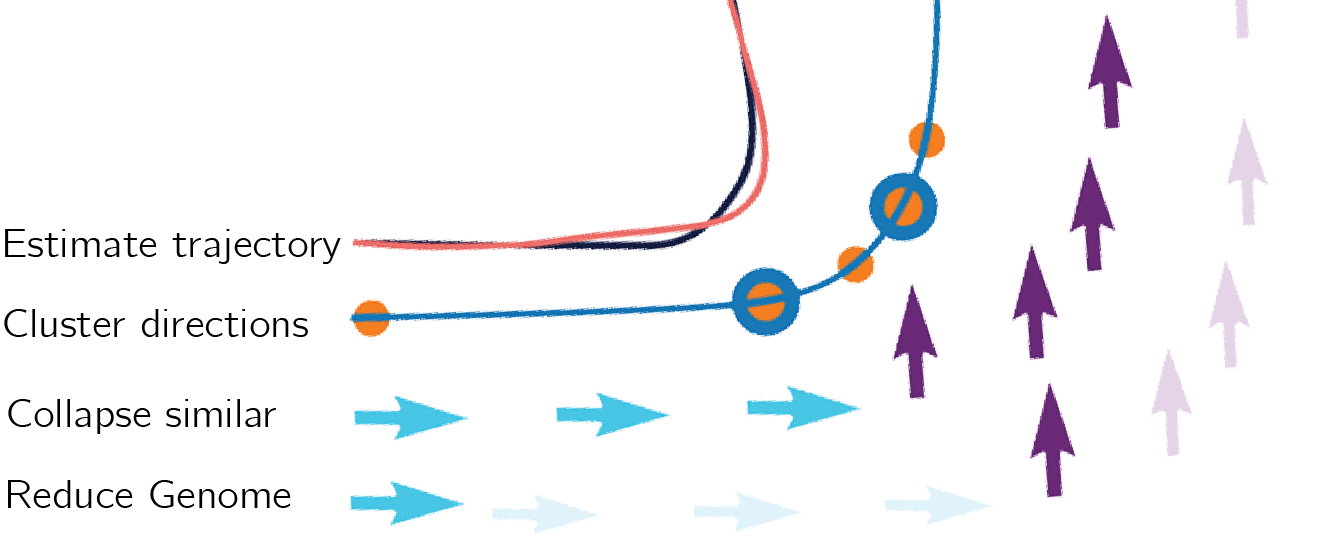
\includegraphics[width=1.0\columnwidth]{img/genome_extract.png}
    \caption{}
    \label{fig:results:genome_extraction}
\end{figure}
\subsubsection{Alignment}
\subsubsection{Fitting}

\subsection{Global Fitting}

\begin{figure}
    \centering
    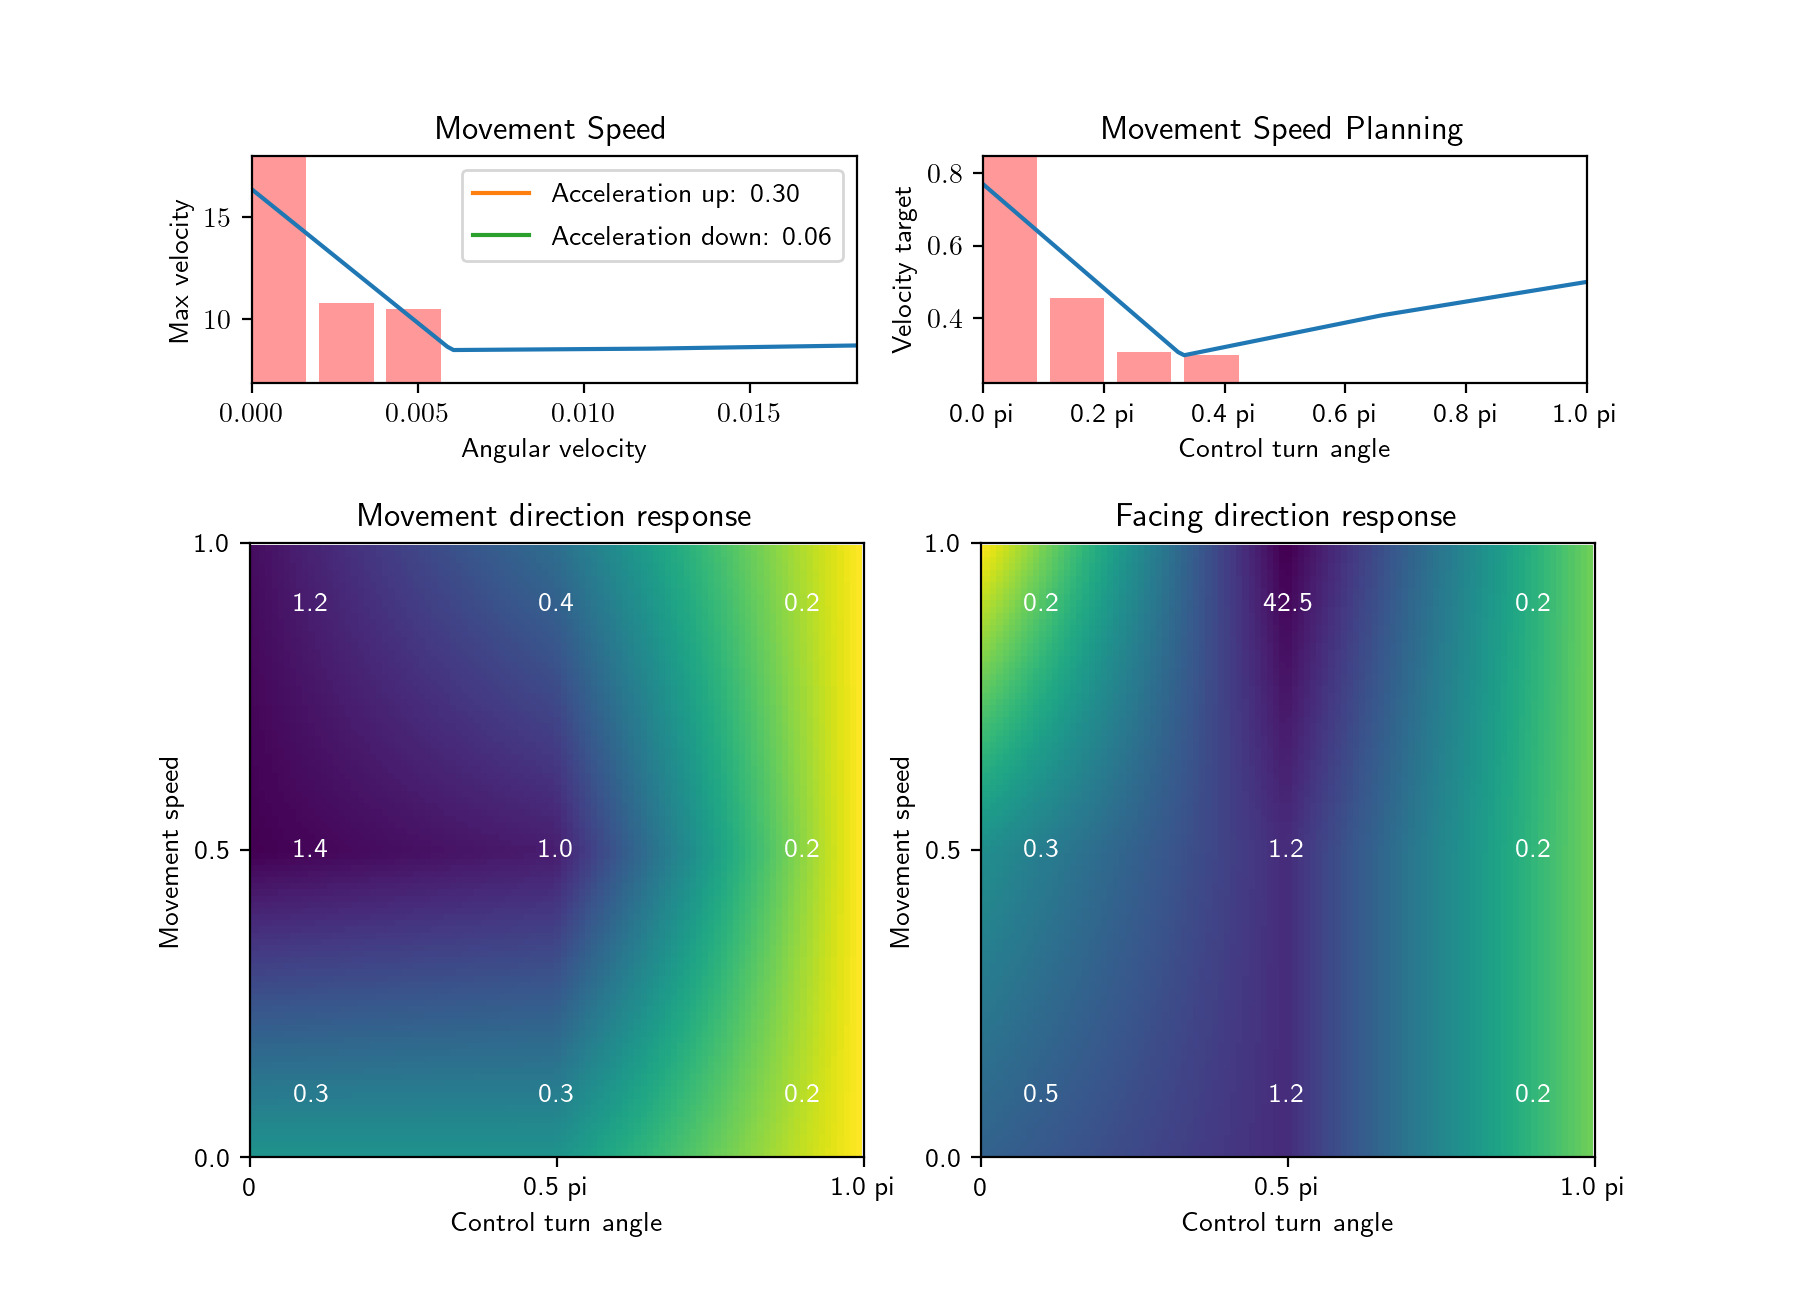
\includegraphics[width=1.0\columnwidth]{img/locomotion mode.png}
    \caption{}
    \label{fig:results:locomotion_mode}
\end{figure}



\section{Video Notes}

\subsubsection{Purpose}
Illustrate the problem we wish to solve using 1-2 video examples.
\subsubsection{Content}
Show that basic animations have complex root motions that are difficult to replicate using standard 'weak control signal' (splines, springs). 
Show that trivial approaches (smoothing) does not solve problem in convincing way.
\paragraph{Videos}
\begin{itemize}
    \item Show character moving straight and in curves. Trace complex root motion. Highlight the presence of both high and low frequency information in the plot.
    \item Show character running straight with smoothed trajectory. Highlight problems. Show turning characters and illustrate how superficially 'identical' turns are actually very different.
\end{itemize}
\paragraph{Figures}
\begin{itemize}
    \item Plots of trajectory and weak control signal paths.
    \item Plots of smoothing effects
\end{itemize}

\subsubsection{Draft}
Final text

\subsection{Fitting Movement Model}
\subsubsection{Purpose} Show that we are able to solve problem using 3-5 video examples (didactic).
Show how various models can be fitted to data (that has itself been adjusted). 
\begin{itemize}
    \item Straight movement. Walk and run. 
    \item Multiple straight movements. Walk and run. 
    \item 180.
    \item Multiple 180s.
    \item Banking
    \item Multiple banking
    \item 45 turn
    \item Multiple 45 turn
    \item 90 turn
    \item Multiple 90 turn
    \item Mixed modes
\end{itemize}
Additionally we could look at animations published by ubisoft.\url{https://github.com/ubisoft/Ubisoft-LaForge-Animation-Dataset}


\subsection{Global Fitting}

\subsection{Application}
\subsubsection{Purpose} Show that our solution has interesting applications using 3-5 video examples (eye candy).
Replace standard control signal with our model.
\begin{itemize}
    \item{Replay animations to illustrate correct root motion}
    \item{Use with motion matching} exponential decay = uttner, Holden Spring damper Kermse 2004].
    \item{use generative neural network} Can we avoid floating character ?
\end{itemize}

